\documentclass{article}
\usepackage[dutch]{babel}
\usepackage[official]{eurosym}
\usepackage{graphicx}
\usepackage{epic,eepic}
\usepackage{mathtools}
\usepackage{caption}
\usepackage{float}
\usepackage{textcomp}
\setcounter{secnumdepth}{5}
\graphicspath{{fig/}}

\makeatletter
\renewcommand\paragraph{%
   \@startsection{paragraph}{4}{0mm}%
      {-\baselineskip}%
      {.5\baselineskip}%
      {\normalfont\normalsize\bfseries}}
\makeatother

\title{Software Design Descriptions voor Schedule-Generator}
\author{Matthias Caenepeel \and Adam Cooman \and Alexander De Cock \and Zjef Van de Poel}
\date{23 februari 2011 Versie 1.0} 

\begin{document}

\maketitle

\newpage

% \newpage
% Signature page

% \newpage

\section*{Aanpassingsgeschiedenis}
\begin{itemize}
\item[.] 23/2/2011 versie 0.1: Aanmaak document \\[-3mm]
\item[.] 27/2/2011 versie 0.2: Toevoeging delen over interfaces \\[-3mm]
\item[.] 28/2/2011 versie 0.3: Toevoeging hoofdstuk over algoritme en Logical \\[-3mm]
\item[.] 28/2/2011 versie 1.0: Verbeteringen doorgevoerd \\[-3mm]
\end{itemize}

%\section*{Preface}

\newpage
\tableofcontents

%\newpage
%\section{Introduction}
%TODO
%\subsection{Purpose}
%\subsection{Scope}
%\subsection{Context}
%\subsection{Summary}

%\newpage
%\section{References}

%\newpage
%\part{Glossary}

\newpage
\section{Body}
\subsection{Identified stakeholders and design concerns}

\subsection{Design viewpoint 1: Compositie}

\subsubsection{Design concerns}
Het doel van dit ontwerpstandpunt bestaat er in alle componenten van het systeem te identificeren, hun attributen te kenmerken en hun onderlinge verbanden te beschrijven. Deze beschrijving zal gebeuren aan de hand van een \textit{component diagram} en het \textit{deployment diagram}. Beide  zijn een onderdeel van de UML 2.0 modelleertaal.  

\subsubsection{Deployment Diagram}

Een deployement diagram geeft weer op welke manier de hard- en software wordt geconfigureerd tijdens de normale werking van het systeem. Hieronder volgt een beschrijving van de belangrijkste componenten in het diagram. 

\begin{figure}[H]%
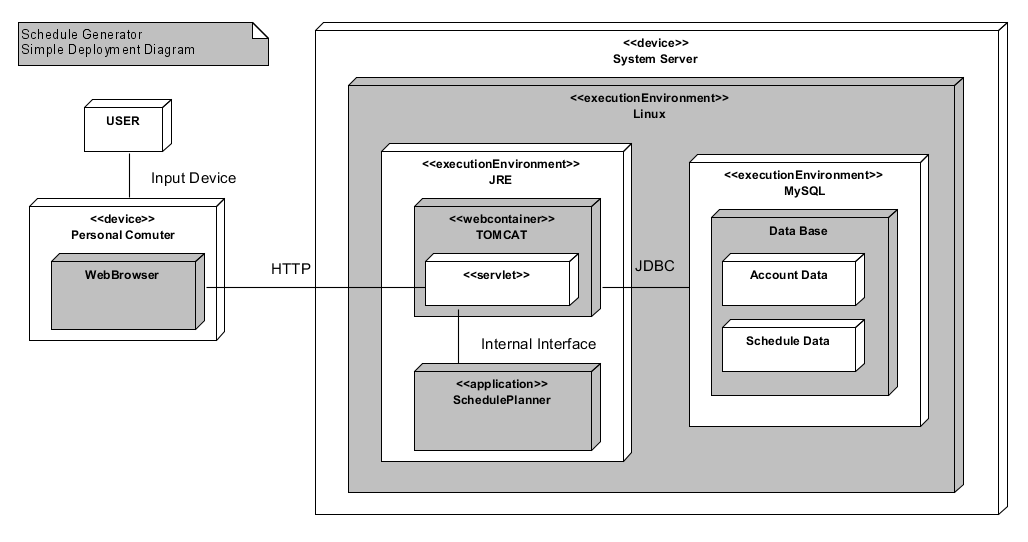
\includegraphics[width=\columnwidth]{DeploymentDiagram.png}%
\caption{Deployment Diagram}%
\end{figure}

\begin{description}

\item[Gebruiker] Een gebruiker die beschikt over een account kan zich aanmelden op de website via zijn gebruikersnaam en wachtwoord. Vervolgens zal hij beschikken over de functionaliteiten, eigen aan zijn gebruikertype. Als de gebruiker geen account heeft kan hij de site betreden als gast. Er wordt dan geen gebruikersgebonden informatie bijgehouden. Meer informatie over de verschillende gebruikertypes en functionaliteiten is voorzien in het SRS. \\
 
\item[Persoonlijke Computer] Toestel dat de hard- en software aan de gebruikerszijde bevat. Er worden geen onderstellingen gemaakt over de eigenschappen van dit toestel met uitzondering dat het instaat is een webbrowser te draaien met eigenschappen gelijkaardig aan die van Internet Explorer, Google Chrome of FireFox.  \\
 
\item[Webbrowser] Er worden geen specifieke onderstelling gemaakt met uitzondering van de reeds vermelde. \\
 
\item[Systeemserver] Tijdens de ontwikkeling van het project wordt Wilma als systeemserver gebruikt. De specificaties van de server worden volledig bepaald door de opdrachtgever en kunnen terug gevonden worden op \\ http://wilma.vub.ac.be/. \\
 
\item[Tomcat] Dit is een webcontainer ontwikkeld door Apache die onder andere toelaat servlets te draaien op een Linux server. Deze servlets zullen de vragen van de gebruiker opvangen en op dynamische wijze webinhoud generen als antwoord. Deze webinhoud zal hoofdzakelijk worden beschreven via XHTML en CVS. Voor meer informatie over Tomcat kan men terecht op \\ http://tomcat.apache.org/. \\
 
\item[Database] De database  maakt onderdeel van de hardware van de systeemserver en bevat zowel de account informatie als de informatie die relevant is voor het opstellen van de lessenroosters. Om gegevens uit de database toegankelijk te maken voor elementen uit de Java runtime environment (JRE) zal gebruikt worden gemaakt van JDBC. Dit is een Java Application Programming Interface ontwikkeld door Sun. Een overzicht wordt gegeven op \\ www.oracle.com/technetwork/java/javase/tech/index-jsp-136101.html

\end{Description}


\subsubsection{Component Diagram}

Zal later worden toegevoegd


%-----------------------------------------------------------------------------------------------------------------------------------------------------

\subsection{Design viewpoint 2: Logical}
\subsubsection{Design concerns}
Om de lessenrooster op te stellen en uit te lezen zijn er verschillende klasses nodig die alle verschillende participerende objecten voorstellen.

\subsubsection{Elementen}
\paragraph{Entiteiten}

\begin{itemize}
	\item[-] Lessen structuur \\[-5mm]
	\begin{itemize}
	  \item[-] \textit{Course}: Les die gevolgd kan worden \\ [-5mm]
	  \item[-] \textit{Subcourse}: Onderdeel van een les; bv hoorcollege, labo of oefeningenles \\[-5mm]
	  \item[-] \textit{Program}: Verzameling van lessen die in een pakket zitten. Bijvoorbeeld 1e bachelor ingenieurswetenschappen \\[-5mm]
	\end{itemize}
	\item[-] Gebouwen strucuur \\[-5mm]
	\begin{itemize}
	  \item[-] \textit{Building}: Gebouw \\[-5mm]
    \item[-] \textit{Room}: Lokaal in een gebouw waar les gegeven kan worden \\[-5mm]
    \item[-] \textit{Hardware}: Materiaal beschikbaar in een lokaal \\[-5mm]
	\end{itemize}
	\item[-] Personen structuur \\[-5mm]
	\begin{itemize}
	  \item[-] \textit{Student}: Persoon die lessen kan volgen \\[-5mm]
    \item[-] \textit{Educator}: Persoon die lessen kan geven; zowel professoren, docenten en assistenten \\[-5mm]
	\end{itemize}
	\item[-] Andere \\[-5mm]
	\begin{itemize}
	  \item[-] \textit{Faculty}: Faculteit van de universiteit \\[-5mm]
	\end{itemize}
\end{itemize}

\paragraph{Relaties}

\begin{itemize}
\item[-] Lessen structuur \\[-5mm]
	\begin{itemize}
	\item[] Elke \textit{Course} bestaat uit een of meerdere \textit{SubCourses} die in opgeteld het gehele vak weergeven. \\[-5mm]
	\item[] \textit{Courses} zelf worden gegroepeerd in een \textit{Program}. \\
	\end{itemize}
\item[-]Gebouwen structuur \\[-5mm]
\begin{itemize}
	\item[] Een gebouw beschikt over een lijst met \textit{Rooms}, die op zich een lijst met beschikbare \textit{Hardware} bijhoudt. \\[-5mm]
	\item[] Een gebouw kan ingedeeld worden onder een faculteit. \\[-5mm]
	\end{itemize}
\item[-] Personen \\[-5mm]
	\begin{itemize}
	\item[] Elke \textit{Student} is ingeschreven in een \textit{Program} en een lijst met afzonderlijke \textit{Courses} die ze volgen.  \\[-5mm]
	\item[] Een \textit{Educator} beschikt over een lijst \textit{Courses} en \textit{SubCourses} die ze geven. \\[-5mm]
\end{itemize}		
\end{itemize}

\paragraph{UML Diagrammma}

\begin{figure}%
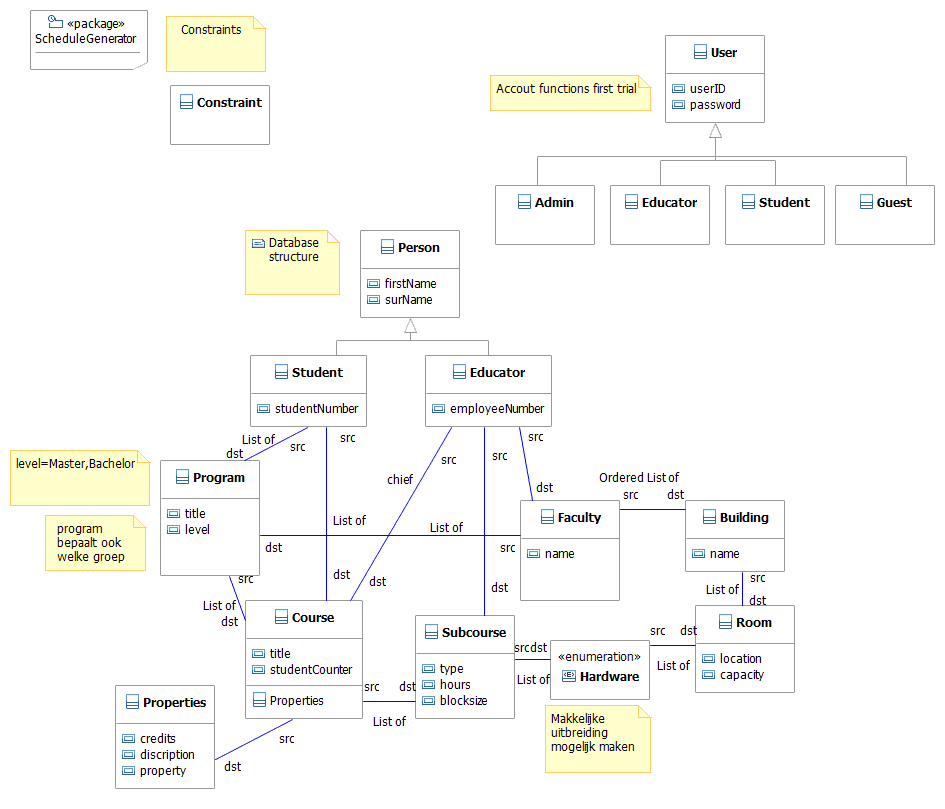
\includegraphics[width=\columnwidth]{UML.png}%
\caption{UML Diagramma}%
\label{UML}
\end{figure}

De klasse waarbij de pijl vertrekt erft van de klasse waar de pijl aankomt. De klasse waarbij er src staat zit in een lijst in de klasse waarbij er dst staat. Zo zit er bijvoorbeeld een lijst van educators in de klasse faculty. \\


\newpage


%------------------------------------------------------------------------------------------------------------------------------------------------------------------


\subsection{Design viewpoint 3: Interfaces}
% HTTP
% Adam schrijft dit het is toegelaten dat je zelf de punten een beke invult

% HTML bestand met javascript om tabs te maken
% HTML bestand met CSS voor layout
% Javascript met CSS intern voor tabber
% HTML met server via HTTP (GET en POST)
% Servlet via interface van Zjef en MySQL met Database

\subsubsection{Design concerns, algemeen}

\begin{figure}[H]
\unitlength=0.3\textwidth
\begin{center}
\begin{picture}(3,1)
%serverlijnen
\put(0.2,0.2){Server}
\put(0.0,0.0){\line(1,0){1.6}}
\put(0.0,0.0){\line(0,1){1.0}}
\put(1.6,0.0){\line(0,1){1.0}}
\put(0.0,1.0){\line(1,0){1.6}}
%browser
\put(2.4,0.2){Browser}
\put(2.2,0.0){\line(1,0){1.6}}
\put(2.2,0.0){\line(0,1){1.0}}
\put(3.8,0.0){\line(0,1){1.0}}
\put(2.2,1.0){\line(1,0){1.6}}
%XHTML
\put(2.32,0.7){Webpagina}
\put(2.4,0.5){XHTML}
\put(2.3,0.9){\line(1,0){0.5}}
\put(2.8,0.4){\line(0,1){0.5}}
\put(2.3,0.4){\line(0,1){0.5}}
\put(2.3,0.4){\line(1,0){0.5}}
%CSS
\put(3.0,0.7){Stylesheet; CSS}
\put(2.95,0.8){\line(1,0){0.8}}
\put(2.95,0.65){\line(0,1){0.15}}
\put(2.95,0.65){\line(1,0){0.8}}
\put(3.75,0.65){\line(0,1){0.15}}
% CSS naar XHTML
\put(2.82,0.725){\line(1,0){0.11}} 
%Javascript
\put(3.0,0.5){Script; Javascript}
\put(2.95,0.6){\line(1,0){0.8}}
\put(2.95,0.45){\line(0,1){0.15}}
\put(2.95,0.45){\line(1,0){0.8}}
\put(3.75,0.45){\line(0,1){0.15}}
% Javascript naar XHTML
\put(2.82,0.525){\line(1,0){0.11}} 
%database
\put(0.15,0.6){Database}
\put(0.1,0.9){\line(1,0){0.5}}
\put(0.6,0.4){\line(0,1){0.5}}
\put(0.1,0.4){\line(0,1){0.5}}
\put(0.1,0.4){\line(1,0){0.5}}
%servlet
\put(1.1,0.8){Servlet}
\put(1.1,0.6){JAVA}
\put(1.0,0.95){\line(1,0){0.5}}
\put(1.5,0.55){\line(0,1){0.4}}
\put(1.0,0.55){\line(0,1){0.4}}
\put(1.0,0.55){\line(1,0){0.5}}
% Files
\put(1.1,0.25){Files}
\put(1.1,0.1){XML}
\put(1.0,0.4){\line(1,0){0.5}}
\put(1.5,0.05){\line(0,1){0.35}}
\put(1.0,0.05){\line(0,1){0.35}}
\put(1.0,0.05){\line(1,0){0.5}}
% lijn Files naar Servlets
\put(1.25,0.42){\line(0,1){0.11}} 
%lijn MySQL
\put(0.65,0.7){MySQL}
\put(0.62,0.65){\line(1,0){0.36}}
%lijn HTTP
\put(1.8,0.7){HTTP}
\put(1.52,0.65){\line(1,0){0.76}}
\end{picture}\\[3mm]
\caption{Overzicht van de verschillende delen van het programma}
\end{center}
\end{figure}

In de structuur van ons programma bestaan verschillende elementen met verschillende taken. Deze moeten met elkaar interageren volgens het bovenstaande schema. De lijnen tussen de verschillende blokken noemen we interfaces en zullen in het volgende deel van het Software Design Document besproken worden. Vooraleer daarmee te beginnen een kort overzicht van de taken die elk blok uit het diagramma uitvoert.

\begin{description}
  \item[Webpagina, XHTML] \hfill \\
  In het XHTML bestand wordt de inhoud van de webpagina geplaatst. 
  \item[Stylesheet, CSS] \hfill \\
  In het stylesheet wordt de lay-out van de webpagina beschreven.
  \item[Script, Javascript] \hfill \\
  In het script word beschreven wanneer welk deel van de webpagina weergegeven wordt. We gebruiken tabbladen om de functionaliteiten die een gebruiker krijgt duidelijk weer te geven. Ht beheer van die tabbladen gebeurt met het javascript "tabber" dat ontwikkeld werd door derden;
  \item[Servlet, JAVA] \hfill\\
  De servlets runnen op tomcat en genereren de XHTML code, afhankelijk van de eigenschappen van de gebruiker.
  \item[Database] \hfill\\
  In de database wordt de informatie van gebruikers en de kalender opgeslaan.
  \item[Files] \hfill\\
  De files bevatten wijzigbare parameters van het programma. Ze zijn in een XML bestand opgeslaan.
\end{description}

Het schema is geen volledig correcte weergave van de werkelijkheid omdat het stylesheet en het script zich ook op de server bevinden en door de browser opgehaald worden van de server via een HTTP protocol. Om volledig correct te zijn zouden die twee onderdelen van het schema zich dus ook op de server moeten bevinden. Om alles overzichtelijk te houden heeft de auteur beslist om ze bij de browser te plaatsen, omdat de browser het ophalen van de server voorziet en niet de gebruiker.

\subsubsection{Interface:  XHTML - CSS voor Layout}
\paragraph{Initialiseren} 

Om het .css bestand aan de XHTML pagina te linken moet in de header van de XHTML code het volgende voorzien worden
\begin{verbatim}
<link rel="stylesheet" href="style.css" type="text/css"> 
\end{verbatim}
Hierin zijn de volgende elementen te herkennen:
\begin{itemize}
\item[] \texttt{rel="stylesheet"}: Duidelijk maken dat de link een link naar een stylesheet is. Deze tag verandert niet \\[-5mm]
\item[] \texttt{type="text/css"}: Duidelijk maken dat de stylesheet in css code geschreven is. Deze tag verandert ook niet \\[-5mm]
\item[] \texttt{href="style.css"}: De naam van het css bestand. Als die zich op een andere locatie bevindt dan de XHTML pagina moet het pad naar die map hierin toegevoegd worden \\[-5mm]
\end{itemize}

\paragraph{Gebruiken} 

In de XHTML code moet niet veel toegevoegd worden om de css op te roepen, enkel een id tag op de volgende manier om onderscheid te maken tussen verschillende gedefini\"{e}erde stijlen in de css code. Als voorbeeld wordt het toevoegen van een id aan een rij van een tabel gegeven om aan te tonen hoe dit moet.
\begin{verbatim}
<tr id="MainBottom">
\end{verbatim}
De naam van het id staat tussen de aanhalingstekens.\\

In het CSS bestand kan de code voor de stijl van hetzelfde id geschreven worden door gebruik te maken van hekje. Als voorbeeld de CSS code die de stijl beschrijfd van de tabelrij uit het vorige voorbeeld.
\begin{verbatim}
tr#MainBottom {
	height:300px;
}
\end{verbatim}

\subsubsection{Interface: XHTML - Javascript voor tabbladen}
\paragraph{Initialiseren} 

Het oproepen van het javascript bestand gebeurt in de header van het XHTML bestand dat de inhoud van de site beschrijft met de volgende code.
\begin{verbatim}
<script type="text/javascript" src="tabber-minimized.js"></script>
\end{verbatim}
Hierin zijn de volgende elementen te herkennen:
\begin{itemize}
\item[] \texttt{type="text/javascript"}: Duidelijk maken dat het javascript is. Deze tag verandert niet \\[-5mm]
\item[] \texttt{src="tabber-minimized.js"}: De naam van het javascript bestand. Als die zich op een andere locatie bevindt dan de HTML pagina moet het pad naar die map hierin toegevoegd worden \\[-5mm]
\end{itemize}

\paragraph{Gebruiken}
Om dan een tabblad aan te maken en er inhoud in te plaatsen wordt gebruik gemaakt van div elementen in de XHTML code. dit gebeurd op de volgende manier:
\begin{verbatim}
<div class="tabber">
<div class="tabbertab" title="Tabblad 1">
Inhoud van het eerste tabblad
</div>
<div class="tabbertab" title="Tabblad 2">
Inhoud van het tweede tabblad
</div>
</div>
\end{verbatim}
In de buitenste div staat het volgenden:
\begin{itemize}
\item[]  \texttt{class="tabber"}: dit vertelt aan het javascript dat er tabbladen volgen. Het laat toe om geneste tabbladen te gebruiken \\[-5mm]
\end{itemize}
In de binnenste divs, \'{e}\'{e}n per tabblad:
\begin{itemize}
\item[] \texttt{class="tabbertab"}: dit vertelt aan het javascript dat er tabbladen volgen. Het laat toe om geneste tabbladen te gebruiken \\[-5mm]
\item[] \texttt{title="Tabblad 1"}: In het title tag staat de titel van het tabblad die bovenaan weergegeven wordt \\[-5mm]
\end{itemize}

\subsubsection{Interface: Javascript - CSS voor tabbladen}

Het Javascript tabber dat gebruikt wordt bevat interne links naar het CSS bestand. De exacte werking van de interface is niet gekend omdat tabber een programma is dat geschreven is door derden. De nodige css code werd aan het stijlbestand toegevoegd zodat alles werk. Het is nu mogelijk om de layout van de tabbladen te defini\"{e}ren in het stijlbestand. De nodige onderverdelingen die toegevoegd moeten worden zijn de volgende:

\begin{verbatim}
.tabberlive .tabbertabhide {}
.tabber {}
.tabberlive {}
ul.tabbernav{}
ul.tabbernav li {}
ul.tabbernav li a {}
ul.tabbernav li a:link {}
ul.tabbernav li a:visited {}
ul.tabbernav li a:hover{}
ul.tabbernav li.tabberactive a{}
ul.tabbernav li.tabberactive a:hover{}
.tabberlive .tabbertab {}
\end{verbatim}


\subsubsection{Interface: Browser - Server: HTTP}

\paragraph{Concerns}
Omdat de algemene kalender en andere gegevens in een database op de server zullen opgeslaan zijn en omdat de gebruiker vanop zijn computer thuis via de website die informatie te zien moet krijgen, moet er een communicatie tussen de server en de browser van de gebruiker zijn. Zoals bij de meeste websites werd gekozen om het het HTTP protocol te werken. We laten niet toe dat de gebruikers rechtstreeks met de database communiceren om te vermijden dat ze informatie te zien krijgen die ze niet mogen zien, en om de informatie op een overzichtelijke manier te structureren. Daarom werken we met Servlets die op server runnen en die de besproken taken verrichten. De volgende paragrafen beschrijven dus de communicatie tussen de browser van de gebruiker en de servlets.

\paragraph{Attributes}

Uit het HTTP protocol zullen de GET en POST functies gebruikt worden door onze toepassing. Een HTTP pakket bestaat uit twee delen, de \textit{header} en de \textit{body}.
\begin{description}
\item[GET] Deze methode vraagt een bepaalde pagina aan de server en zet alles in de \textit{header}. Het is de methode die gebruikt wordt bij het klikken op een link van een site. Deze zal dus de meest gebruikte methode zijn om te communiceren met de server. \\
\item[POST] Deze methode stuurt informatie door in de \textit{body} van het paket.\\
\end{description}
De manier waarop de informatie doorgestuurd zal worden hangt af van de plaats. Gevoelige informatie, zoals wachtwoorden zal via een POST verzonden worden, omdat de header gemakkelijk zichtbaar is voor gebruikers. Lange informatie, zoals beschrijvingen van vakken zal ook via de POST methode verzonden worden, omdat de lengte van de \textit{header} beperkt is. \\

Andere informatie, zoals het opvragen van het lessenrooster zal via de GET methode gebeuren. De waarden van de zoekactie worden dan in de link geplaatst door een script dat nog ontwikkeld moet worden en waarvan de interface met de XHTML pagina gelijkenissen zal vertonen met die voor de tabbladen. \\

We gebruiken HttpServlets die de doGet methode bevatten om een Get aanvraag binnen te krijgen en die te beantwoorden. Beschouw als voorbeeld de volgende servlet. Hij stuurt het antwoord Hallo terug naar de gebruiker als die de juiste URL ingegeven heeft. Welke URL dat is wordt beschreven in een XML bestand dat zich op de server bevindt en een bepaalde URL aan een Servlet koppelt.

\begin{verbatim}
public class test2 extends HttpServlet {
public void doGet(HttpServletRequest request,
                  HttpServletResponse response)
  throws ServletException, IOException {
    response.setContentType("text/html");
    PrintWriter out = response.getWriter();
    out.println("Hallo");
  }
}	
\end{verbatim}

Het gebruik van de POST methode wordt op dit moment nog onderzocht door het team en zal binnenkort verduidelijkt worden.


\subsubsection{Interface: Database interface}

\paragraph{Concerns}
De interface met de MySQL database, bevattende alle objecten beschreven in 2.1, dient op een algemene manier aangesproken te kunnen worden vanuit de andere onderdelen van het project.

\paragraph{Elementen}

\begin{itemize}
\item[-] Database \\[-5mm]
\begin{itemize}
\item[-] \textbf{Database}: Handle naar de database. Levert methodes om tabellen in te lezen, opzoekingen te 		doen, objecten weg te schrijven en dergelijke.
\item[-] \textbf{Table}: Een enkele tabel uit de database
\item[-] \textbf{Element}: Een element van een tabel
\end{itemize}		
\item[-] Interface \\[-5mm]
\begin{itemize}
\item[-] \textbf{Databasable}: Inteface* die duidelijk maakt dat een object van een klasse die 	\textit{Databasable} implementeert, in de database geschreven, of uit de database gelezen 	kan worden. \\[-5mm]
\item[-] \textbf{InDatabase}: Annotation* die duidelijk maakt dat een bepaalde parameter van een object in de 		database bewaard moet worden. \\[-5mm]
\item[-] \textbf{OutDatabase}: Annotation* die duidelijk maakt dat een bepaalde parameter van een object  uit de 		database gelezen en naar het object gekopieerd moet worden. \\[-5mm]
\end{itemize}		
\end{itemize}		
		
*: Java terminologie

\subsubsection{Interface: File interface}

\paragraph{Concerns}
Wijzigbare parameters moeten opgeslagen worden in een file. Hiervoor wordt gebruik gemaakt van XML. Deze interface biedt de mogelijkheid om vanuit het programma eenvoudige XML bestanden uit te lezen en aan te maken.

\paragraph{Elementen}

\begin{itemize}
\item[-] \textbf{XMLDocument}: Object verwijzende naar een XML bestand. Een XMLDocument bevat een lijst van 	XMLElement \\[-5mm]
\item[-] \textbf{XMLElement}: Element van een XML bestand. Een element heeft een bepaalde waarde, of bevat zelf een 	aantal andere elementen. \\[-5mm]
\begin{itemize}
	\item[-] \textbf{ElementWithValue}: Element met een waarde \\[-5mm]
	\item[-] \textbf{ElementWithChildren}: Element met lijst van andere elementen, zijn \textit{Children}.(\textit{Children} kunnen op hun beurt ook weer \textit{ElementWithChildren} of \textit{ElementWithValue} zijn) \\[-5mm]
\end{itemize}		
\item[-] \textbf{XMLParser}: Levert methodes om een XML bestand, gecre�erd met deze interface, weer in te laden naar 	een XMLDocument 
\end{itemize}

\paragraph{Schema}

\begin{figure}[H]
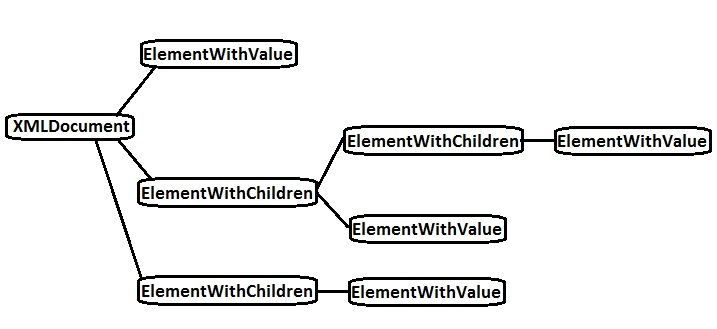
\includegraphics[width=\columnwidth]{XML.png}%
\caption{Voorbeeld van een \textit{XMLDocument}}%
\end{figure}

\newpage

%-----------------------------------------------------------------------------------------------------------------------------------------------------------------

\subsection{Design viewpoint 4: Algoritme voor kalenderplanning}
% Matthias schrijft dit wel
\subsubsection{Design concerns}

Het algoritme dient in staat te zijn om een lessenrooster te maken dat aan bepaalde voorwaarden (constraints) voldoet. Het is daarom belangrijk dat deze eerst bepaald worden. Men kan een indeling maken in deze voorwaarden. Zo zijn er de \textit{fixed} constraints aan deze moeten zeker voldaan zijn, anders klopt het lessen rooster niet. \textit{Hard constraints} deze moeten zo goed mogelijk vervuld zijn en dan zijn er nog \textit{soft constraints} deze staan onderaan de ladder en hoeven dus niet noodzakelijk vervuld te zijn. Aan de hand van deze voorwaarden kan men dan nagaan hoe goed het lessenrooster is. Dit doet men aan de hand van een \textit{fitnessvalue}. Zo krijgt een geplaatste les 3 punten als aan een \textit{fixed constraint} voldaan is, 2 voor een hard en 1 voor een soft. Aangezien de \textit{fixed constraints} zeker voldaan moeten zijn, moet een geplaatste les al zeker 12 punten hebben. Op die manier kan men het resultaat evalueren.

\begin{itemize}
\item[] \textit{Fixed constraints}\\[-3mm]
\begin{enumerate}
	\item Er mag nooit meer dan 1 les gepland zijn in een leslokaal \\[-3mm]
	\item Een docent (educator) kan niet meer dan 1 les geven  \\[-3mm]
	\item Een leslokaal (room) moet groot genoeg zijn voor het aantal studenten \\[-3mm]
	\item Als een les bepaald materiaal vereist (zoals computer, laboratorium,...) moet hier aan worden tegemoet gekomen. \\[-3mm]
\end{enumerate}
\item[] \textit{Hard constraints} \\[-3mm]
\begin{enumerate}
 \item Het lessenrooster van een student mag niet overlappen. \\[-3mm]
 \item Er mag van een vak bijvoorbeeld hoogstens 4 uur per dag gegeven worden. \\[-3mm]
 \item Student mogen bijvoorbeeld maximum 8 uur les per dag krijgen. \\[-3mm]
\end{enumerate}
\item[] \textit{Soft constraints} \\[-3mm]
\begin{enumerate}
 \item De werkcolleges mogen pas na of gelijktijdig met de theoriecolleges beginnen. \\[-3mm]
\end{enumerate}
\end{itemize}

Voor iedere week van het academisch jaar zal de lessenrooster een tabel bevatten voor elke student die bestaat uit 5 dagen (maandag t.e.m. vrijdag) waar voor elke dag de uren bijstaan (er kan les gegeven worden van 8u t.e.m. 18u). \\

Het algoritme zal deze tabel in een eerste fase zo opbouwen dat er aan de fixed constraints voldaan is en dan in een tweede fase proberen om de totale fitnessvalue op te drijven.

\subsubsection{Design elements}

Om het algoritme te kunnen uitvoeren is er natuurlijk de nodige informatie nodig om tot een lessenrooster te kunnen komen. De informatie die nodig is, zal uit een database worden gehaald en dan in klassenstructuur gegoten worden. Deze klassenstructuur is besproken in "Design Viewpoint 2: Logical".
Het schema en bijbehorende uitleg kan daar gevonden worden.
Deze structuur zal nog worden uitgebreid met methode die de rooster opstellen en dan hieruit vertrekkende de fitnessvalue bepalen. De bovenstaande structuur zal met andere woorden nog worden uitgebreid.

%\subsection{Design rationale}


%\begin{figure}
%\begin{center}
%\includegraphics[width=\textwidth]{Bangladesh}
%\caption*{Bangladesh}
%\end{center}
%\end{figure}

%\begin{tabular}[t]{llll}
%Mandi & Katholiek & 25\% & Platte neus -- spleetogen \\
%Gohli & Moslims   & 75\% & Grote ogen -- scherpere neus \\
%Kooch & Hindu     & 1\%  & Mengeling van de twee \\
%\end{tabular}
%\\[5mm]

%\begin{itemize}
%\item[.] Slaapmatje \\[-3mm]
%\item[.] Kleren: 3 korte broeken, 6 onderbroeken, 4 T-shirts\\[-3mm]
%\item[.] Longi: voor 's avonds en als pyjama\\[-3mm]
%\item[.] Tandenborstel en twee tubes tandpasta\\[-3mm]
%\end{itemize}


 \end{document}